% HeadProbe -- PerCom-style paper (IEEE conference template, two-column, US letter).
%
% STATUS: DRAFT. No participant data exist yet. Every result number is a red placeholder (\ph{...}).
% The results text is written in the direction the hypotheses predict. When the data are in,
% rewrite each results sentence to what was actually found -- including null or opposite results --
% and delete \draftbanner. Numbers that are NOT placeholders are design parameters of the app or
% come from the scorer self-test (analysis/headprobe_analyze.py --selftest), and are real.
\documentclass[conference,letterpaper]{IEEEtran}
\IEEEoverridecommandlockouts
% IEEEtran asks for Times. pdfLaTeX (Overleaf's default) has it built in; XeTeX/Tectonic does not,
% so use the TeX Gyre Termes clone there. pdfLaTeX output is unchanged.
\usepackage{iftex}
\ifXeTeX
  \usepackage{fontspec}
  \setmainfont{texgyretermes}[Extension=.otf, UprightFont=*-regular, BoldFont=*-bold,
    ItalicFont=*-italic, BoldItalicFont=*-bolditalic]
\fi
\usepackage{cite}
\usepackage{amsmath}
\usepackage{graphicx}
\usepackage{booktabs}
\usepackage{xcolor}
\usepackage{tikz}
\usetikzlibrary{arrows.meta,positioning,calc}
\usepackage[hidelinks]{hyperref}

% Placeholders and notes. Search the PDF for red text before submitting.
\newcommand{\ph}[1]{\textcolor{red}{#1}}
\newcommand{\todo}[1]{\textcolor{red}{[TODO: #1]}}
\newcommand{\draftbanner}{\textcolor{red}{\textbf{DRAFT -- all participant results in red are placeholders; no data have been collected.}}}
\newcommand{\figph}[2]{\fbox{\parbox[c][#1][c]{0.94\linewidth}{\centering\footnotesize\textcolor{red}{Placeholder figure:}\\ #2}}}

\begin{document}

\title{HeadProbe: Measuring Mental Load and Drowsiness\\ from Head Turns toward Spatial Sounds on Earbuds}

% Single-blind venue: real names and affiliations go here.
\author{\IEEEauthorblockN{\todo{Author names}}
\IEEEauthorblockA{\todo{Department, institution, city, country}\\
\todo{email addresses}}}

\maketitle

\begin{abstract}
\draftbanner{}
Reaction-time probes are the most trusted objective measures of mental load and alertness, but they
need a button, a screen or lab equipment, so they are rarely used where overload and fatigue happen.
We present HeadProbe, which runs such a probe on commodity earbuds. A short sound is rendered from a
random direction with spatial audio, the user turns their head toward it, and the earbuds' motion
sensor measures how quickly the turn starts, whether it happens at all, and where it lands. The head
turn leaves the hands and eyes free and adds a measure a button cannot give: the accuracy and
left--right bias of the turn. In a load study (\ph{N=XX}), head-turn latency rose with n-back
difficulty as reliably as the standard button-press Detection Response Task (\ph{XX} vs.\ \ph{XX}
ms from 0- to 3-back) and agreed with it per block (\ph{r = X.XX}). In a drowsiness study
(\ph{N=XX}), misses and latency increased with self-rated sleepiness, and misses grew more for sounds
on the left (\ph{XX\%} vs.\ \ph{XX\%}), mirroring the rightward attention shift known from
laboratory studies of sleep onset. Ordinary earbuds can thus measure load and drowsiness hands-free.
\end{abstract}

\begin{IEEEkeywords}
earables, spatial audio, cognitive load, drowsiness, detection response task, head tracking
\end{IEEEkeywords}

\section{Introduction}
Overload and fatigue cause errors at work, on the road and in study, yet they are hard to measure
where they occur. Questionnaires such as NASA-TLX~\cite{hart2006nasa} or the Karolinska Sleepiness
Scale~\cite{akerstedt1990subjective} are filled in afterwards, interrupt the person, and rely on
self-report. Physiological sensing needs extra hardware and is noisy in motion. The most trusted
objective measures are \emph{probe reaction times}: the Detection Response Task (DRT) for cognitive
load, standardised as ISO~17488~\cite{iso17488}, and the Psychomotor Vigilance Test (PVT) for
alertness~\cite{dinges1985microcomputer,basner2011maximizing}. Both work by the same principle:
a task that consumes attention leaves less spare capacity for noticing a probe, so responses slow
down or are missed~\cite{kahneman1973attention,wickens2008multiple}. Both, however, need a response
button, and the DRT standard itself warns that the manual response can conflict with manual tasks.

Earbuds are worn for hours a day, can place a sound anywhere around the head with spatial audio,
and many now contain a motion sensor that tracks the head~\cite{roddiger2022sensing,
ferlini2019head,apple2020headphonemotion}. This makes them a natural probe device. We propose
HeadProbe: a brief sound plays from a random direction and the user turns their head toward it.
The turn replaces the button, so the hands and eyes stay free. It also carries more information than
a button press. A button records \emph{when} the probe was noticed; a head turn also records
\emph{where} the user believed the sound came from, and how directly they got there. Spatial
judgements are known to shift with drowsiness: as people fall asleep, sounds on the left are missed
and mislocalised more often~\cite{bareham2014losing,jagannathan2022decreasing}.

This paper asks whether head turns toward spatial sounds, measured by commodity earbuds, can stand
in for the established probe methods. We contribute:
\begin{itemize}
\item HeadProbe, an iOS system that renders spatial probes on AirPods, scores head turns from the
  earbuds' head tracking (onset latency, misses, endpoint error, side), and runs a button-press
  reference with identical probes. The scorer is validated in simulation.
\item A load study comparing head-turn and button responses across n-back levels.
\item A drowsiness study testing whether head-turn misses, latency and left--right bias track
  self-rated sleepiness.
\end{itemize}

\begin{figure*}[t]
\centering
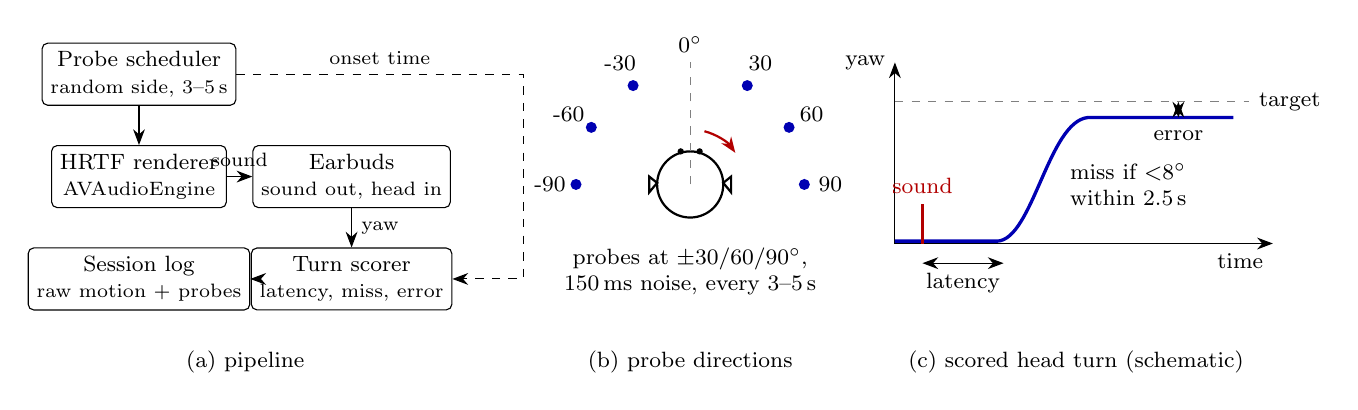
\begin{tikzpicture}[font=\footnotesize, >={Stealth[length=2mm]},
    box/.style={draw, rounded corners=2pt, align=center, minimum height=0.75cm, inner sep=3pt}]
  % (a) pipeline
  \begin{scope}[xshift=-7.0cm, yshift=0.1cm]
    \node[box] (sched) at (0,1.3) {Probe scheduler\\ \scriptsize random side, 3--5\,s};
    \node[box] (hrtf) at (0,0) {HRTF renderer\\ \scriptsize AVAudioEngine};
    \node[box] (buds) at (2.7,0) {Earbuds\\ \scriptsize sound out, head in};
    \node[box] (score) at (2.7,-1.3) {Turn scorer\\ \scriptsize latency, miss, error};
    \node[box] (log) at (0,-1.3) {Session log\\ \scriptsize raw motion + probes};
    \draw[->] (sched) -- (hrtf);
    \draw[->] (hrtf) -- node[above] {\scriptsize sound} (buds);
    \draw[->] (buds) -- node[right] {\scriptsize yaw} (score);
    \draw[->] (score) -- (log);
    \draw[->,dashed] (sched.east) -| node[pos=0.25,above] {\scriptsize onset time} ([xshift=9mm]score.east) -- (score.east);
    \node at (1.35,-2.35) {(a) pipeline};
  \end{scope}
  % Left: top view of the head and probe directions.
  \begin{scope}
    \draw[thick] (0,0) circle (0.42);
    \fill (-0.12,0.42) circle (0.04); \fill (0.12,0.42) circle (0.04); % eyes = front
    \draw[thick] (0.42,0.02) -- (0.52,0.1) -- (0.52,-0.1) -- cycle;    % right ear
    \draw[thick] (-0.42,0.02) -- (-0.52,0.1) -- (-0.52,-0.1) -- cycle; % left ear
    \draw[dashed,gray] (0,0) -- (0,1.55) node[above,black] {0$^\circ$};
    \foreach \a in {-90,-60,-30,30,60,90} {
      \fill[blue!70!black] ({90-\a}:1.45) circle (0.07);
      \node at ({90-\a}:1.78) {\a};
    }
    \draw[->,thick,red!70!black] (75:0.7) arc (75:35:0.7);
    \node[align=center] at (0,-1.1) {probes at $\pm$30/60/90$^\circ$,\\ 150\,ms noise, every 3--5\,s};
    \node at (0,-2.25) {(b) probe directions};
  \end{scope}
  % (c) schematic yaw trace with the scored measures.
  \begin{scope}[xshift=2.6cm,yshift=-0.75cm]
    \draw[->] (0,0) -- (4.8,0) node[below left] {time};
    \draw[->] (0,0) -- (0,2.3) node[left] {yaw};
    \draw[dashed,gray] (0,1.8) -- (4.5,1.8);
    \node[anchor=west] at (4.5,1.8) {target};
    \draw[very thick,blue!70!black] (0,0.03) -- (1.3,0.03)
         .. controls (1.75,0.05) and (1.95,1.55) .. (2.45,1.6) -- (4.3,1.6);
    \draw[red!70!black,thick] (0.35,0) -- (0.35,0.5) node[above] {sound};
    \draw[<->] (0.35,-0.25) -- (1.38,-0.25) node[midway,below] {latency};
    \draw[<->] (3.6,1.6) -- (3.6,1.8);
    \node[anchor=north] at (3.6,1.55) {error};
    \node[align=left,anchor=west] at (2.1,0.75) {miss if $<$8$^\circ$\\ within 2.5\,s};
    \node at (2.3,-1.5) {(c) scored head turn (schematic)};
  \end{scope}
\end{tikzpicture}
\caption{HeadProbe. (a) The phone schedules a probe, renders it from a random side, and scores the
head turn from the earbuds' motion data. (b) Probe directions relative to the head at sound onset.
(c) Latency runs from sound onset to the turn crossing 2$^\circ$; the endpoint is where the first
movement stops; error is its distance from the target.}
\label{fig:overview}
\end{figure*}

\section{Related Work}
\subsection{Probe-based measures of load and vigilance}
In the DRT, a light, vibration or sound appears every 3--5\,s while the participant performs a
primary task, and they press a button as fast as possible; reaction time and hit rate increase with
the task's cognitive load~\cite{iso17488,strayer2015assessing}. The PVT measures sustained attention
with a simple reaction task and is highly sensitive to sleep loss, mainly through lapses
($>$500\,ms) and slowing~\cite{dinges1985microcomputer,basner2011maximizing}; an auditory PVT
behaves like the visual one under sleep deprivation~\cite{jung2011comparison}. All of these use a
manual response and no spatial information. HeadProbe keeps their logic and timing but replaces
the stimulus with a spatialised sound and the response with a head turn.

\subsection{Head orienting to sound}
Pointing the head at a sound is a standard measure of localisation~\cite{makous1990two}.
Lertpoompunya et al.~\cite{lertpoompunya2024head} tracked head turns toward speech in a
loudspeaker array during a dual task. Listeners undershot targets beyond 60$^\circ$, and under the
hardest listening conditions paused before turning (``wait-and-listen''). That work studies
hearing, with lab loudspeakers and optical tracking; we use the turn as a probe of a separate task's
load, on earbuds. Spatial audio menus selected by head gestures go back to Brewster et
al.~\cite{brewster2003multimodal}, and pointing at spatial audio targets degrades with
mobility~\cite{marentakis2006effects}. AudioPIN uses AirPods head tracking and spatial sounds for
authentication~\cite{naitou2026audiopin}. A patent describes a headset that checks whether its wearer
turns toward a loud ambient sound to decide whether to warn them~\cite{samsung2024ambient}; it does
not estimate load or alertness.

\subsection{Spatial attention, drowsiness and earables}
Bareham et al.\ found that as people drift toward sleep, errors in judging the side of a sound rise
for the left, a rightward shift of spatial attention~\cite{bareham2014losing}, later linked to
perceptual decision-making under decreasing alertness~\cite{jagannathan2022decreasing}. Those studies
used button responses and EEG-defined drowsiness in the lab. Under everyday circadian fatigue, by
contrast, Minton et al.\ found faster notice times and no change in VR sound-pointing
error~\cite{minton2025longitudinal}. Earable drowsiness detection has so far relied on in-ear
EEG~\cite{kaveh2024wireless} or motion patterns~\cite{roddiger2022sensing}, not on responses to a
probe. To our knowledge, no work uses earbud-measured head turns toward spatial probes to measure
load or drowsiness.

\section{HeadProbe}

\subsection{Probe design}
Each probe is a 150\,ms burst of broadband noise with 5\,ms ramps, identical on every trial as in
the DRT. Broadband noise carries the high-frequency cues that spatial rendering relies on. The burst
is rendered with Apple's head-related transfer function (HRTF) renderer at one of six azimuths,
$\pm$30$^\circ$, $\pm$60$^\circ$ and $\pm$90$^\circ$ relative to where the head points at onset
(Fig.~\ref{fig:overview}). We use only lateral positions: a generic HRTF localises front and back
poorly~\cite{wenzel1993localization}, and a sound straight ahead needs no turn. Directions are drawn
without replacement, so each appears once per cycle of six. Onsets follow each other every 3--5\,s
(uniform), as in the DRT, and a response counts within 2.5\,s. The burst ends before a head turn
can start, so no head-tracked re-rendering is needed during playback. The participant is instructed
to turn toward each sound as quickly as possible and then face forward again. The instruction
matters: an uninstructed orienting response habituates to a repeated, meaningless sound.

\subsection{Head tracking and scoring}
Head orientation comes from AirPods through Apple's headphone motion
interface~\cite{apple2020headphonemotion} at about 25\,Hz (\ph{XX.X\,Hz measured}). A one-time
calibration (face forward, then turn right) fixes the zero direction and the sign of yaw. Because
earbud yaw drifts slowly, every probe is scored relative to the median yaw in the 300\,ms before
onset. The scorer finds the first sample beyond 8$^\circ$ within the window. If there is none, the
probe is a \emph{miss}. Otherwise, \emph{latency} is the interpolated time at which yaw last rose
through 2$^\circ$ before that point, and starts under 100\,ms are flagged as anticipations. The
\emph{endpoint} is the yaw where angular speed first stays below 20$^\circ$/s for two samples; the
\emph{error} is endpoint minus target, and \emph{side} records whether the first turn went toward
the sound. Gaps over 250\,ms in the motion stream mark the probe as unscorable.
Table~\ref{tab:measures} summarises the measures and what each is meant to capture.

\begin{table}[t]
\caption{Measures scored per probe and per block.}
\label{tab:measures}
\centering
\footnotesize
\setlength{\tabcolsep}{3pt}
\begin{tabular}{@{}p{0.2\linewidth}p{0.47\linewidth}p{0.27\linewidth}@{}}
\toprule
Measure & Definition & Construct \\
\midrule
Latency & onset to 2$^\circ$ crossing (median per block) & speed of noticing, as DRT/PVT \\
Miss & no turn beyond 8$^\circ$ within 2.5\,s & lapse, as DRT/PVT \\
Lapse & latency above a per-person threshold & PVT-style lapse \\
$|$Error$|$ & $|$endpoint $-$ target$|$ & localisation quality \\
Side bias & left minus right miss rate; mean signed error & spatial attention shift \\
Wrong side & first turn away from the sound & gross mislocalisation \\
\bottomrule
\end{tabular}
\end{table}

\subsection{Timing}
Motion samples, touch events and audio scheduling share one clock (the system's monotonic host
time). The sound onset is the scheduled host time plus the output latency the system reports plus a
Bluetooth offset that the system does not report. We measure that offset with a sync mode that plays
a click and flashes the screen at the same scheduled instant, filmed at 240 frames/s with an
earbud at the camera's microphone. On our AirPods Pro 2 the offset was \ph{XXX $\pm$ XX\,ms}
(\ph{n = XX} clicks). Its variability bounds the precision of latency; misses, lapses and turn
accuracy do not depend on it.

\subsection{Implementation and scorer validation}
HeadProbe is a SwiftUI app for iOS~17 (AVAudioEngine with an environment node for rendering, Core
Motion for head tracking). It logs every raw motion sample, so all measures are recomputed offline
by an analysis script that implements the same scorer. A \emph{tap} mode presents identical probes
and records touches on the screen with their hardware timestamps, giving a button-press reference.
We validated the scorer on 540 simulated minimum-jerk head turns sampled at 25\,Hz with random
sample phase and 0.3$^\circ$ noise, toward all six targets and with latencies of 250, 450 and
800\,ms. Latency was within 15\,ms of the true crossing time in every case. Endpoint errors of
$-$15$^\circ$ and $+$12$^\circ$ (undershoot, overshoot) were recovered within 0.1$^\circ$, and
across 50 simulated still heads with 1.5$^\circ$ noise no turn was falsely detected.

\section{Technical Evaluation}
Before the user studies, we characterised the hardware and the baseline accuracy of earbud head
turns, because these bound what the studies can detect.

\textbf{Motion stream.} Over \ph{XX} minutes of logging on AirPods Pro~2 with an iPhone
\ph{XX}, motion samples arrived at \ph{XX.X\,Hz} (interval \ph{XX.X $\pm$ X.X\,ms}); \ph{X.X\%} of
intervals exceeded twice the mean, and \ph{X.X\%} of probes in the studies below were unscorable
because of gaps.

\textbf{Audio timing.} The Bluetooth offset measured with the sync mode was \ph{XXX $\pm$ XX\,ms}
over \ph{XX} clicks in \ph{X} sessions; the reported output latency was \ph{XX\,ms}. A standard
deviation of \ph{XX\,ms} is \ph{small/large} relative to the load effects reported for the
DRT~\cite{strayer2015assessing}, so we report latency \ph{as means and as lapses}.

\textbf{Localisation baseline.} \ph{XX} participants, seated with no other task, responded to
120 head-turn probes (20 per direction). Turns went to the correct side on \ph{XX.X\%} of probes.
Endpoints undershot the target with increasing eccentricity (mean endpoint \ph{XX$^\circ$},
\ph{XX$^\circ$} and \ph{XX$^\circ$} for 30, 60 and 90$^\circ$; Fig.~\ref{fig:baseline}), as
expected for head pointing~\cite{makous1990two,lertpoompunya2024head}, and median latency was
\ph{XXX\,ms}. Because undershoot is systematic, the studies compare errors between conditions
within each direction rather than against the nominal target.

\begin{figure}[t]
\centering
\figph{2.8cm}{Endpoint yaw vs.\ target azimuth (six directions), per participant and mean,\\
with the identity line; inset: latency distribution.}
\caption{Localisation baseline: where earbud-measured head turns land for each probe direction.
\ph{Placeholder.}}
\label{fig:baseline}
\end{figure}

\section{Study 1: Mental Load}
\subsection{Design}
\ph{XX} participants (\ph{XX} women, age \ph{XX $\pm$ XX}) performed a visual n-back task on a
laptop, with letters every 2.5\,s, at four levels (0-, 1-, 2- and 3-back), a standard graded
working-memory load~\cite{owen2005nback}. Each level was run twice, once with head-turn responses
and once with tap responses, in 3-minute blocks, giving 8 blocks in counterbalanced order after
practice. Probes ran throughout. After each block, participants completed NASA-TLX as a
manipulation check. Because a head turn takes the eyes off the screen, we also measure the probe's
cost to the primary task: n-back accuracy on letters shown during a probe's response window.

\noindent\textbf{Hypotheses.} H1: head-turn latency and misses increase with n-back level.
H2: head-turn latency agrees with tap latency across blocks. H3: turn accuracy degrades with load.
H4: head-turn probes cost the primary task more than tap probes.

\noindent\textbf{Analysis.} Linear mixed models with n-back level as a fixed effect and participant
as a random intercept, per measure; agreement by repeated-measures correlation of block medians and
Bland--Altman limits.

\subsection{Results}
\begin{table}[t]
\caption{Study 1: median latency (ms), misses (\%) and absolute turn error by n-back level.
Mean $\pm$ SD over participants. \ph{All values are placeholders.}}
\label{tab:load}
\centering
\setlength{\tabcolsep}{4pt}
\begin{tabular}{@{}lcccc@{}}
\toprule
& 0-back & 1-back & 2-back & 3-back \\
\midrule
Tap latency     & \ph{XXX $\pm$ XX} & \ph{XXX $\pm$ XX} & \ph{XXX $\pm$ XX} & \ph{XXX $\pm$ XX} \\
Head latency    & \ph{XXX $\pm$ XX} & \ph{XXX $\pm$ XX} & \ph{XXX $\pm$ XX} & \ph{XXX $\pm$ XX} \\
Tap misses      & \ph{X.X} & \ph{X.X} & \ph{X.X} & \ph{X.X} \\
Head misses     & \ph{X.X} & \ph{X.X} & \ph{X.X} & \ph{X.X} \\
Head $|$error$|$ ($^\circ$) & \ph{XX.X} & \ph{XX.X} & \ph{XX.X} & \ph{XX.X} \\
NASA-TLX        & \ph{XX} & \ph{XX} & \ph{XX} & \ph{XX} \\
\bottomrule
\end{tabular}
\end{table}

\begin{figure}[t]
\centering
\figph{3.2cm}{Median latency vs.\ n-back level, head turn and tap, with 95\% CIs (left);\\
Bland--Altman plot of head vs.\ tap block medians (right).}
\caption{Study 1: head-turn and tap latency across load levels, and their agreement.
\ph{Placeholder.}}
\label{fig:load}
\end{figure}

NASA-TLX rose with n-back level (\ph{F(3, XX) = XX.X, p < .001}), confirming the manipulation.
Head-turn latency increased from \ph{XXX} ms at 0-back to \ph{XXX} ms at 3-back
(\ph{F(3, XX) = XX.X, p < .001}; Table~\ref{tab:load}, Fig.~\ref{fig:load}), as did tap latency
(\ph{XXX} to \ph{XXX} ms, \ph{F(3, XX) = XX.X, p < .001}), supporting H1. The effect of load was
\ph{comparable} in size for both responses (0- vs.\ 3-back: \ph{$d_z$ = X.XX} head, \ph{$d_z$ =
X.XX} tap). Head turns were on average \ph{XXX} ms slower than taps, a constant offset: block
medians correlated at \ph{$r_{rm}$ = X.XX}, and the Bland--Altman bias was \ph{XXX} ms with limits
of agreement \ph{$\pm$XXX} ms (H2). Misses rose from \ph{X.X\%} to \ph{X.X\%}. Absolute turn error
\ph{increased} with load, from \ph{XX.X}$^\circ$ to \ph{XX.X}$^\circ$
(\ph{F(3, XX) = X.X, p = .XXX}; H3), and all participants undershot $\pm$90$^\circ$ targets
(\ph{mean endpoint XX$^\circ$}), consistent with~\cite{lertpoompunya2024head}. N-back accuracy on
letters during a response window was \ph{X.X} points lower with head turns than with taps
(\ph{p = .XXX}; H4).

\section{Study 2: Drowsiness}
\subsection{Design}
\ph{XX} right-handed participants (the leftward effect was reported for right-handers) took part in
one 45-minute session in the early afternoon. They reclined in a dimly lit room with eyes closed and
no task other than responding to head-turn probes, a setting that lets drowsiness develop without
sleep deprivation. Every 5 minutes a recorded voice asked for a Karolinska Sleepiness Scale rating
(1--9), given aloud~\cite{akerstedt1990subjective}. A 5-minute tap-mode PVT-style block at the start
and end gives a button-press reference.

\noindent\textbf{Hypotheses.} H5: misses and latency increase with sleepiness rating.
H6: misses and signed error shift toward the right (more left misses) as sleepiness rises.

\noindent\textbf{Analysis.} Mixed models of each measure on the most recent rating, with probe side
(left or right) and its interaction for H6.

\subsection{Results}
\begin{figure}[t]
\centering
\figph{3.0cm}{Miss rate (top) and median latency (bottom) vs.\ Karolinska Sleepiness rating,\\
separately for left and right probes, with 95\% CIs.}
\caption{Study 2: head-turn misses and latency by sleepiness and probe side. \ph{Placeholder.}}
\label{fig:drowsy}
\end{figure}

Sleepiness ratings rose from \ph{X.X} to \ph{X.X} over the session. Each point on the scale raised
the miss rate by \ph{X.X} percentage points (\ph{p < .001}) and latency by \ph{XX} ms
(\ph{p < .001}), supporting H5 (Fig.~\ref{fig:drowsy}). The increase in misses was larger for left
probes than for right probes (side $\times$ sleepiness, \ph{p = .XXX}): at ratings of 7 or more,
\ph{XX\%} of left and \ph{XX\%} of right probes were missed. Signed error shifted rightward by
\ph{X.X}$^\circ$ per scale point (\ph{p = .XXX}; H6). Tap reaction times slowed from the first to
the last reference block by \ph{XX} ms (\ph{p = .XXX}).

\section{Discussion}
\textbf{Earbuds can run a probe test.} \ph{If H1--H2 hold:} head-turn latency followed load as the
button-press DRT did, with a constant offset, so earbuds already worn for hours can provide the
standard measure without a button or screen. \ph{If H5--H6 hold:} the same probes tracked
sleepiness, and the left--right asymmetry reported in the lab~\cite{bareham2014losing} appeared in
earbud head turns, a spatial measure a button cannot give.

\textbf{Applications.} The most direct use is as a field instrument for researchers who need load or
alertness during real tasks. Workers who already wear headsets for a whole shift, such as call-centre
or control-room operators, could take short fatigue checks without extra devices. Repeated at-home
checks could help track fatigue in health conditions where it fluctuates.

\textbf{Limitations.} A head turn takes the eyes away, so HeadProbe suits seated or listening tasks,
not driving or walking, where turning is unsafe. Generic HRTFs limit accuracy, which is why probes
are lateral. Bluetooth latency adds variance to latency; we report misses and errors that do not
depend on it. The probe interrupts, as every probe method does, and repeated sounds invite
habituation. Study 2's drowsiness was self-rated, not EEG-defined, and ordinary fatigue may not shift
spatial judgements~\cite{minton2025longitudinal}. Both samples were small and from
\ph{one university}.

\textbf{Ethics.} Both studies were approved by \ph{the institutional review board of XX (protocol
XX)}. No sleep deprivation was induced.

\section{Conclusion}
HeadProbe turns commodity earbuds into a hands-free, screen-free probe of mental load and
drowsiness. A sound from a random direction and the head turn toward it give latency and misses that
\ph{track} the established button-press measures, plus turn accuracy and left--right bias that
buttons cannot provide. Next, we will \ph{test HeadProbe during everyday seated work, compare it with
ear-EEG, and study how often probes can be played before users habituate or object}.

\bibliographystyle{IEEEtran}
\bibliography{refs}

\end{document}
